\documentclass[tikz,border=10pt]{standalone}
\begin{document}
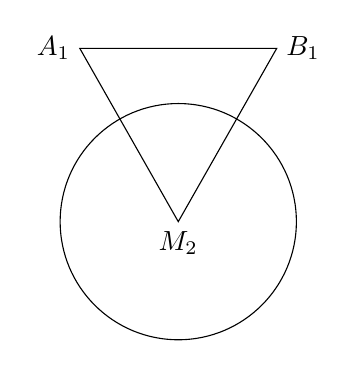
\begin{tikzpicture}
    % --- 参数定义 ---
    \def\radius{1.5}      % 圆的半径
    \def\triHeight{2.2}   % 三角形高度
    \def\triWidth{2.5}    % 三角形底边宽度

    % --- 绘制圆 ---
    \draw (0,0) coordinate (M2) circle (\radius);
    \node[below] at (M2) {$M_2$};

    % --- 绘制三角形 ---
    % 定义三个顶点
    \coordinate (A1) at (-\triWidth/2, \triHeight/1);
    \coordinate (B1) at (\triWidth/2, \triHeight/1);
    
    % 绘制路径
    \draw (M2) -- (A1) node[left] {$A_1$} -- (B1) node[right] {$B_1$} -- cycle;

\end{tikzpicture}
\end{document}